\section{Реализация}

Программная реализация выполнена в Jupyter Notebook \code{lab02.ipynb} на языке
\textit{Python}. Для воспроизводимости был зафиксирован \code{SEED = 7}. В
ноутбуке отдельно реализованы функции для VIF-фильтрации, построения dummy-
переменных, генерации банка нелинейных функций, восстановления состояний и
обучения классификатора.

Основные параметры финального запуска:
\begin{codebox}
\begin{lstlisting}[language=Python]
SEED = 7
VIF_MAX = 8.0
SPEARMAN_MIN = 0.40
R2_MIN = 0.70
REG_ALPHA = 1.0
LOGREG_C = 8.0

USE_SPHERE_IN_STATE_MODELS = True
USE_COMMUNITY_IN_STATE_MODELS = False
USE_SPHERE_IN_CLASSIFIER = True
USE_COMMUNITY_IN_CLASSIFIER = False
\end{lstlisting}
\end{codebox}

В known-части содержится 1900 наблюдений, в unknown-части --- 600 наблюдений.
Состояния для unknown-строк отсутствуют полностью, поэтому они восстанавливались
отдельной регрессионной моделью, обученной на known-части.

\begin{figure}[H]
    \centering
    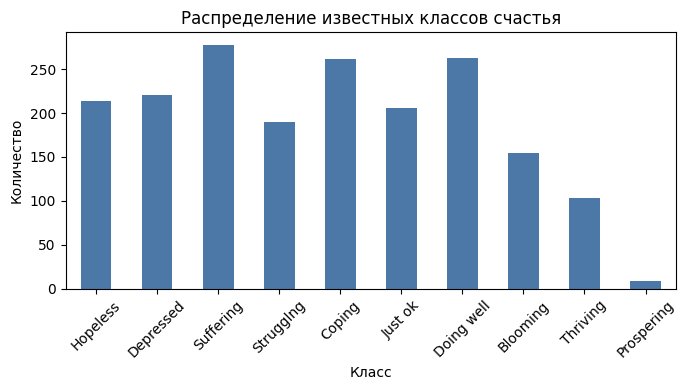
\includegraphics[width=0.86\textwidth]{images/class_distribution.png}
    \caption{Распределение классов счастья в known-части}
    \label{fig:class_dist}
\end{figure}

Распределение классов несбалансировано. Особенно редко встречается класс
\textit{Prospering}: в known-части всего 9 таких наблюдений. Это ограничивает
устойчивость оценок для верхнего края шкалы и частично объясняет ошибки между
соседними категориями.

\newpage
